\documentclass[onecolumn,10pt,cleanfoot]{asme2ej}

\usepackage{graphicx} %% for loading jpg figures
\usepackage{bm}
\usepackage{nicefrac}
\usepackage{mathtools}
\usepackage{amssymb}
\usepackage{amsmath}
\usepackage{parskip}
\usepackage{listings}
\usepackage{tablefootnote}
\usepackage{float}
\usepackage{xcolor}
\usepackage{xurl}
\usepackage{tikz}
\usepackage{caption}
\usepackage{hyperref}

\author{Grzegorz Kajda
    \affiliation{
	Bachelor Student, Robotics and Intelligent Systems\\ \\[-10pt]
	Department of Informatics The faculty of Mathematics and Natural Sciences\\ \\[-10pt]
    Email: grzegork@ifi.uio.no
    }
}


\begin{document}
\title{Constructing a Convolutional Neural Network from ground up}
\maketitle

\section{Abstract}

To gain a more comprehensive understanding of the inner mechanisms of deep learning networks, we developed a Convolutional Neural Network (CNN) from scratch for image classification. The network is structured into two main parts: a feed-forward network and a filtering network consisting of convolutional and pooling layers. Fortunately, we had previously built a feed-forward neural network as part of the subject "FYS-STK3155" at the University of Oslo. Hence, we utilized this code as a foundation for our new network.

To enhance the modularity and resemblance to deep learning libraries like TensorFlow and PyTorch, we modularized the architecture of our network. Instead of having the entire network in one module, we created separate modules representing different types of layers. This approach enables us to construct flexible architectures in a simple and transparent manner while emphasizing the blackbox concept.

Finally, we evaluated the performance of our initial implementation of a CNN using the 28x28 MNIST dataset, which served as a test benchmark.

\section{Introduction}
Machine Learning, particularly the sub-branch known as deep learning, has emerged as a powerful tool for data analysis and classification in the contemporary world. It enables us to extract meaningful insights from data with minimal effort and automate tasks like data clustering or generating new data from existing sources. With the advent of deep learning libraries such as TensorFlow and Keras, this process has become even simpler, allowing data scientists and developers to focus solely on their specific tasks without concerning themselves with the implementation details of these algorithms. While this "blackbox" approach saves valuable time, it can limit our understanding of how the algorithms truly work. Consider the example of backpropagation: deep learning libraries utilize automatic differentiation, eliminating the need to manually compute or propagate gradients backwards from the output to input. However, without referring to external resources, it is unlikely that one would be able to implement the algorithm from scratch.

To gain a deeper understanding of how data is processed and transformed layer by layer, we will develop a Convolutional Neural Network (CNN) from scratch. This endeavor aims to draw insightful conclusions about the inner workings of the network. While prioritizing the blackbox ideology mentioned earlier, we will also ensure that the code is accessible and more readable than that of existing Machine Learning APIs.

Before delving into the theoretical aspects of this project, it is important to note that we assume the reader is already familiar with concepts such as backpropagation in feed-forward networks and the use of schedulers for optimizing gradient descent. If these concepts are unfamiliar, we highly recommend reading our previous paper, which provides a detailed explanation of implementing a feed-forward network, including backpropagation and how it is affected by the use of various activation and cost functions. The paper can be found at: \href{https://github.com/EricEReber/FFNN_optimization/blob/main/doc/paper.pdf}{\color{blue}Neural networks for solving regression and classification problems}.

\section{Theory}

\subsection{Description of structure}
When building a standalone neural network from scratch, a common approach is to encapsulate the code within a single method or class. Typically, the architecture is defined by providing a list of integer values, where the length of the list indicates the number of hidden layers, and the values within the list specify the dimensions of each layer. While this approach is acceptable, it can sometimes be counterintuitive and prone to errors. In our implementation, we opt for a more organized approach by dividing the code into manageable modules called "layers." These layers serve as explicit representations of the individual layers within the neural network.

Similar to TensorFlow, we instantiate these layers, which automatically add them to a list in the order they are created. This allows for easy comparison with the functionality provided by existing machine learning libraries. The list containing our layers is stored within a container class called \textbf{CNN}. Additionally, the \textbf{CNN} class includes additional functionality for controlling all layers simultaneously.

Having discussed the general structure of our code, we will now describe each type of layer that we will be using and explain their functionalities.

\subsection{Fully connected layer}
\subsubsection{Forward pass}
The fully connected layer, as the name suggests, represents a standard layer type commonly found in feed-forward neural networks. In the feed-forward mode, this layer takes a batch of data as input and performs a batch-weight matrix multiplication. The resulting product is then passed through an activation function, which elevates the weighted input into a higher-dimensional encoding. This process enables the network to learn arbitrary relationships between the input data's features. The key difference is that instead of using a for loop to iterate over each layer, we explicitly pass data from one layer to another.

Mathematically, we can define the action of this layer using the following equation:

\begin{equation}
a_i^l = f^l(z_i^l) = f^l\left(\sum_{j=1}^{N_{l-1}} w_{ij}^l a_j^{l-1} + b_i^l\right).
\end{equation}

Where the variables are defined as follows: $a_i^l$ represents the activation of the $i$-th neuron in layer $l$, $f^l(\cdot)$ denotes the activation function specific to layer $l$, $z_i^l$ is the weighted sum of inputs for neuron $i$ in layer $l$, $w_{ij}^l$ represents the weight connecting neuron $j$ in layer $l-1$ to neuron $i$ in layer $l$, $a_j^{l-1}$ is the activation of neuron $j$ in layer $l-1$, and $b_i^l$ is the bias term for neuron $i$ in layer $l$. This equation captures the essential computation performed by the fully connected layer, where input data is transformed into a higher-level representation using a combination of weighted sums and activation functions, and then propagated forward to the next layer.

\subsubsection{backward pass}
When it comes to backpropagation, the principles remain the same, and only our method of encapsulation has changed. By applying the chain rule repeatedly, we can iteratively calculate the gradient for each layer, starting from the output layer and working our way backward. This process, known as reverse mode of automatic differentiation, is computationally preferable over forward mode, where we begin at the input layer \cite[416]{sr}. The equations used for gradient calculation in a feed-forward neural network (FFNN), which we will not derive here, are as follows \cite{morten}:

First, we calculate the delta terms for all layers, beginning with the output layer:

\begin{equation}
y_i^l = f^l(u_i^l) = f^l\left(\sum_{j=1}^{N_{l-1}} w_{ij}^l y_j^{l-1} + b_i^l\right).
\end{equation}

We then utilize this term in an iterative process, moving backward through the network with the following equation:

\begin{equation}
\delta_j^l = \sum_k \delta_k^{l+1}w_{kj}^{l+1}f'(z_j^l).
\end{equation}

Using these delta terms, we can compute the gradients for the weights and biases in each layer:

\begin{gather}
w_{jk}^l\leftarrow = w_{jk}^l- \eta \delta_j^la_k^{l-1}, \
b_j^l \leftarrow b_j^l-\eta \frac{\partial {\cal C}}{\partial b_j^l}=b_j^l-\eta \delta_j^l.
\end{gather}

These equations demonstrate how the gradients are updated for the weights $w_{jk}^l$ and biases $b_j^l$ in each layer, where $\eta$ represents the learning rate, $\delta_j^l$ is the delta term for neuron $j$ in layer $l$, and $a_k^{l-1}$ denotes the activation of neuron $k$ in the previous layer. By iteratively updating these gradients, we optimize the network's parameters and enhance its ability to learn and make accurate predictions. 

\subsection{Two types}
The fully connected layers are split into two classes; FullyConnectedLayer which acts as a hidden layer, and OutputLayer, which acts as the single output layer at the end of the CNN. If one wishes to use this codebase to construct a normal feed forward neural network, it must start with a FlattenLayer due to techincal details regarding weight intitialization. However many FullyConnectedLayers can be added to the CNN, and in each layer the amount of nodes, which activation function and scheduler to use can be specified. In practice, the scheduler will be specified in the CNN object initialization, and inherited if no other scheduler is specified.

\subsection{Convolution}
In order to construct a convolutional neural network (CNN), it is crucial to comprehend the fundamental principles of convolution and how it aids in extracting information from images. Convolution, at its core, is merely a mathematical operation between two functions that yields another function. It is represented by an integral between two functions, which is typically expressed as:

\begin{equation}
(f \ast g)(t) := \int_{-\infty}^{\infty} f(\tau) g(t-\tau) d \tau
\end{equation}

Here, f and g are the two functions on which we want to perform an operation. The outcome of the convolution operation is represented by $(f \ast g)$, and it is derived by sliding the function g over f and computing the integral of their product at each position. If both functions are continuous, convolution takes the form shown above. However, if we discretize both f and g, the convolution operation will take the form of a sum between the elements of f and g:

\begin{equation}
(f \ast g)[n] = \sum_{m=0}^{n-1} f[m] g[n-m]
\end{equation}

The key idea we utilize to extract the information contained in an image is to slide an $m \times n$ matrix *g* over an $m \times n$ matrix \textit{f}. In our case, \textit{f} represents the image, while \textit{g} represents the kernel, oftentimes called a filter. However, since our convolution will be a two-dimensional variant, we need to extend our mathematical formula with an additional summation:

\begin{equation}
(f \ast g)[i, j] = \sum_{m=0}^{M-1} \sum_{n=0}^{N-1} f[m,n] g[i-m, j-n]
\end{equation}

It is imperative to note that the size of the kernel g is significantly smaller than the size of the input image f, thereby reducing the amount of computation necessary for feature extraction. Furthermore, the kernel is usually a trainable parameter in a convolutional neural network, allowing the network to learn appropriate kernels for specific tasks. Now to give you an example of how 2D convolution works in practice, suppose we have an image \textit{f} of dimension $6 \times 6$

\begin{equation}
f = \begin{bmatrix}
4 & 1 & 2 & 9 & 8 & 6 \\
9 & 5 & 9 & 5 & 8 & 5 \\
1 & 5 & 9 & 7 & 6 & 4 \\
2 & 9 & 8 & 3 & 7 & 1 \\
8 & 1 & 6 & 4 & 2 & 2 \\
1 & 0 & 5 & 7 & 8 & 2 \\
\end{bmatrix}
\end{equation}

and a $3 \times 3$ kernel \textit{g} called a low-pass filter. Note that the kernel is usually rotated by 180 degrees during convolution, however this has no effect on this kernel

\begin{equation}
g = \frac{1}{9} \begin{bmatrix}
1 & 1 & 1 \\
1 & 1 & 1 \\
1 & 1 & 1 \\
\end{bmatrix}
\end{equation}

In order to filter the image, we have to extract a $3 \times 3$ element from the upper left corner of \textit{f}, and perform element-wise multiplication of the extracted image pixels with the elements of the kernel \textit{g}:
\begin{equation}
\begin{bmatrix}
4 & 1 & 2 \\
9 & 5 & 9 \\
1 & 5 & 9 \\
\end{bmatrix}
\cdot
\begin{bmatrix}
\frac{1}{9} & \frac{1}{9} & \frac{1}{9} \\
\frac{1}{9} & \frac{1}{9} & \frac{1}{9} \\
\frac{1}{9} & \frac{1}{9} & \frac{1}{9} \\
\end{bmatrix}
=
\begin{bmatrix}
\frac{4}{9} & \frac{1}{9} & \frac{2}{9} \\
\frac{9}{9} & \frac{5}{9} & \frac{9}{9} \\
\frac{1}{9} & \frac{5}{9} & \frac{9}{9} \\
\end {bmatrix}
= \textbf{A}
\end{equation}

Then, following the multiplication, we summarize all the elements of the resulting matrix A:

\begin{equation}
(f \ast g)[0, 0] = \sum_{i=0}^{2} \sum_{j=0}^{2} a_{i,j} = 5
\end{equation}

Which corresponds to the first element of the filtered image $(f \ast g)$.

	Here we use a stride of 1, a parameter denoted \textit{s} which describes how many indexes we move the kernel \textit{g} to the right before repeating the calculations above for the next $3 \times 3$ element of the image \textit{f}. It is usually presumed that \textit{s=1}, however, larger values for *s* can be used to reduce the dimentionality of the filtered image such that the convolution operation is more computationally efficient. In the context of a convolutional neural network, this will become very useful.

The full result of the convolution is: 

\begin{equation}
\begin{bmatrix}
5 & 5.78 & 7 & 6.44 \\
6.33 & 6.67 & 6.89 & 5.11 \\
5.44 & 5.78 & 5.78 & 4 \\
4.44 & 4.78 & 5.56 & 4 \\
\end{bmatrix}
\end{equation}

The result is markedly smaller in shape than the original image. This occurs when using convolution without first padding the image with additional columns and rows, allowing us to keep the original image shape after sliding the kernel over the image. How many rows and columns we wish to pad the image with depends strictly on the shape of the kernel, as we wish to pad the image with r additional rows and c additional columns.

\begin{equation}
r = \left\lfloor \frac{{\text{{kernel height}}}}{2} \right\rfloor \cdot 2 \\
c = \left\lfloor \frac{{\text{{kernel width}}}}{2} \right\rfloor \cdot 2
\end{equation}

Note the notation $\lfloor \frac{kernel width}{2} \rfloor$ means that we floor the result of the division, meaning we round down to a whole number in case $\frac{kernel width}{2}$ results in a floating point number.
Using those simple equations, we find out by how much we have to extend the dimensions of the original image. Before proceeding, however, we might ask what we shall fill the additional rows and columns with? One of the most common approaches to padding is zero-padding, which as the name suggest, involves filling the rows and columns with zeros. This is the approach that we will be using for this demonstration. If we apply this padding to out original $6 \times 6$ image, the result will we an $8 \times 8$ image as the kernel has a width and height of 3. Note that the original image is encapsuled by the zero-padded rows and columns:

\begin{equation}
\begin{bmatrix}
0 & 0 & 0 & 0 & 0 & 0 & 0 & 0 \\
0 & 4 & 1 & 2 & 9 & 8 & 6 & 0 \\
0 & 9 & 5 & 9 & 5 & 8 & 5 & 0 \\
0 & 1 & 5 & 9 & 7 & 6 & 4 & 0 \\
0 & 2 & 9 & 8 & 3 & 7 & 1 & 0 \\
0 & 8 & 1 & 6 & 4 & 2 & 2 & 0 \\
0 & 1 & 0 & 5 & 7 & 8 & 2 & 0 \\
0 & 0 & 0 & 0 & 0 & 0 & 0 & 0 \\
\end{bmatrix}
\end{equation}

\subsubsection{Fun fact}
When filtering images, you will see that convolution involves rotating the kernel by 180 degrees. However, this is not the case when applying convolution in a CNN, where the same operation not rotated by 180 degrees is called cross-correlation.

\subsection{Convolution2DLayer: convolution in a hidden layer}
After establishing the foundational understanding of applying convolution to spatial data, let us delve into the intricate workings of a convolutional layer in a Convolutional Neural Network (CNN). The primary function of convolution, as previously discussed, is to extract pertinent information from images while simultaneously decreasing the scale of our data. To initiate the image processing, we shall begin by partitioning the images into color channels (unless the image is grayscale), comprising three primary colors: red, green, and blue. We will subsequently utilize trainable kernels to construct a higher-dimensional encoding of each channel called feature maps. Successive layers will receive these feature maps as inputs, generating further encodings, albeit with reduced dimensions. The term trainable kernels denotes the initialization of pre-defined kernel-shaped weights, which we will then train via backpropagation, similar to how weights are trained in a Feedforward Neural Network.

To ensure seamless integration between our implementation of the convolutional layer and popular machine learning frameworks like Tensorflow (Keras) and PyTorch, we have adopted a design pattern that mirrors the construction of models using these APIs. This involves implementing our convolutional layer as a Python class or object, which allows for a more modular and flexible approach to building neural networks. By structuring our code in this way, users can easily incorporate our implementation into their existing machine learning pipelines without having to make significant changes to their codebase. Additionally, this design pattern promotes code reusability and makes it easier to maintain and update our convolutional layer implementation over time. 

Note that the Convolution2DLayer takes in an activation function as a parameter, as it also performs non-linearity.

\subsubsection{Backpropagation in the convolutional layer}
As you may have noticed, we have not yet explained how the backpropagation algorithm works in a convolutional layer. However, having covered all other major details about convolutional layers, we are now prepared to do so. It should come as no surprise that the calculation of delta terms at each convolutional layer takes the form of convolution. After the gradient has been propagated backwards through the flattening layer, where it was reshaped into an appropriate form, calculating the update value for the kernel is simply a matter of convolving the output gradient with the input of the layer for which we are updating the weights. For more detail, this article serves as an excellent resource \href{https://pavisj.medium.com/convolutions-and-backpropagations-46026a8f5d2c}{\color{blue}Convolutions\ and\ backpropagations}

\subsubsection{Format of input data}
Note that image data usually comes in many different shapes and sizes, but for our CNN we require the input data be formatted as [Number of inputs, input channels, input height, input width]. Occasionally, the data you come accross use will be formatted like this, but on many occasions reshaping and transposing the dimensions is sadly necessary.

\subsection{Optimized Convolution2DLayer}
or our CNN, we have also implemented an optimized version of the Convolution2DLayer (following guidance from [Weidman, A. Deep Dives], although many modifications had to be made), Convolution2DLayerOPT, which runs much faster. See VII. Remarks for discussion. This layer will per default be used by the CNN due to its computational advantages, but is much less readable. We've documented it such that specially interested students can understand the principles behind it, but it is not recommended to read. In short, we reshape and transpose parts of the image such that the convolutional operation can be swapped out for a simple matrix multiplication.

\subsection{Pooling Layer}
The pooling layer is a commonly used layer in convolutional neural networks (CNNs) that facilitates downsampling of data to a more manageable size. Despite advancements in convolution techniques that preserve data size, the pooling layer remains a fundamental component of CNNs. It can be positioned before, after, or between convolutional layers, and the optimal arrangement and network depth depend on experimental evaluation to achieve the best performance for a given problem. Our provided code allows for two types of pooling: max pooling and average pooling. In max pooling, the value of a pixel at coordinates $(x,y)$ is determined by selecting the maximum value among the pixels in a window extracted in the same manner as before convolution. On the other hand, average pooling extracts the window and computes the new pixel's intensity as the average intensity of the pixels in that window.

\subsection{Flattening Layer}
Before we can begin building our first CNN model, we need to introduce the flattening layer. As its name suggests, the flattening layer transforms the data into a one-dimensional vector that can be fed into the feedforward layers of our network. This layer plays a crucial role in preparing the data for further processing in the network. Additionally, the flattening layer is responsible for reshaping the gradient to the proper shape during backpropagation. This ensures that the kernels are correctly updated, allowing for effective learning in the network.

\subsection{Datasets} 

\subsubsection{MNIST}
The MNIST dataset is a well known multiclass classification problem used to test machine learning algorithms. It consists of $70000$ black and white images of hand drawn digits, each $28$ by $28$ pixels. Each image is labeled with one of ten classes, corresponding to the digit it depicts. The dataset is divided into $60000$ training images and $10000$ test images. This dataset is essentially uniformly distributed, with all classes containing around $9 - 11\%$ of the total dataset.

\subsubsection{CIFAR-10}
CIFAR-10 is widely recognized as one of the most commonly used datasets for benchmarking image classification models. Consisting of $60000$ RGB pictures, it encompasses 10 distinct classes, such as airplanes, automobiles, and dogs. Similar to the MNIST dataset, CIFAR-10 maintains a uniform distribution among the classes, with approximately $6000$ examples per class. However, it should be noted that the images within this dataset possess relatively low resolution. This low resolution further compounds the challenges inherent in classifying objects that have inherent physical disparities, such as distinguishing between transportation vehicles and animals.

\subsection{Note}
All the theoretical concepts discussed, as well as the corresponding code for each component described, including the convolutional layer, pooling layer, and the CNN itself, are presented in a comprehensive Jupyter Notebook file here: \href{https://github.com/EricEReber/CNN/blob/main/doc/CNN_in_Python.ipynb}{\color{blue}CNN\ in\ Python}. The notebook provides detailed explanations and examples on how to use these components to build a fully functioning CNN. It serves as a valuable resource for understanding and implementing convolutional neural networks.

\section{Results}
With the theory and implementation explained, we can now discuss the results we achieved by applying our CNN to the datasets introduced above. 

\subsection{CNN on MNIST}
It is widely acknowledged that standard convolutional neural networks (CNNs) exhibit remarkable performance, rivaling human cognitive abilities, particularly in recognizing hand-written digits. Surprisingly, achieving such results does not require complex architectures with multiple layers. In line with this understanding, our initial architecture comprises a solitary convolutional layer with one input and one output channel. The layer employs a symmetric kernel with dimensions of 2x2 and a stride of 3 in both the horizontal and vertical directions. Following this convolutional layer, we include a flattening layer, which is succeeded by two fully connected layers. These layers utilize the Leaky ReLU function as their activation unit and consist of 30 and 20 hidden nodes, respectively. The final layer, serving as the output layer, contains 10 nodes, facilitating multiclass classification using softmax activation. Despite its simplicity, this architecture yields impressive results, with a training accuracy of approximately 99\% and a validation accuracy ranging from 97\% to 98\%, all achieved without employing any form of grid search. A plot of accuracy over epochs and the confusion matrix for the predictions using $\textit{xval}$ dataset are provided below. (There seems to be something small errors in the confusion matrix, as accuracy computed from the matrix is a couple percent lower than that computed using method $np.average(y_{pred} == y_{val})$):

\begin{figure}[H]
  \centering
	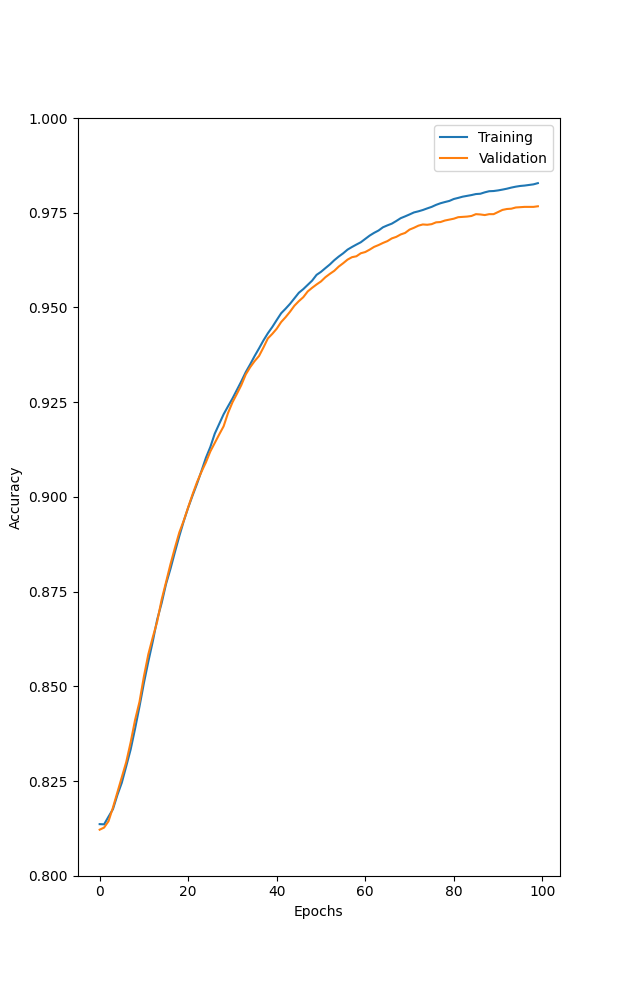
\includegraphics[width=0.9\textwidth, height=0.75\textwidth]{mnist28_trainVal_acc.png}
	\caption{Development of the prediction accuracy with the progression of epochs}
  \label{fig:MINST_acc}
\end{figure}

\begin{figure}[H]
  \centering
	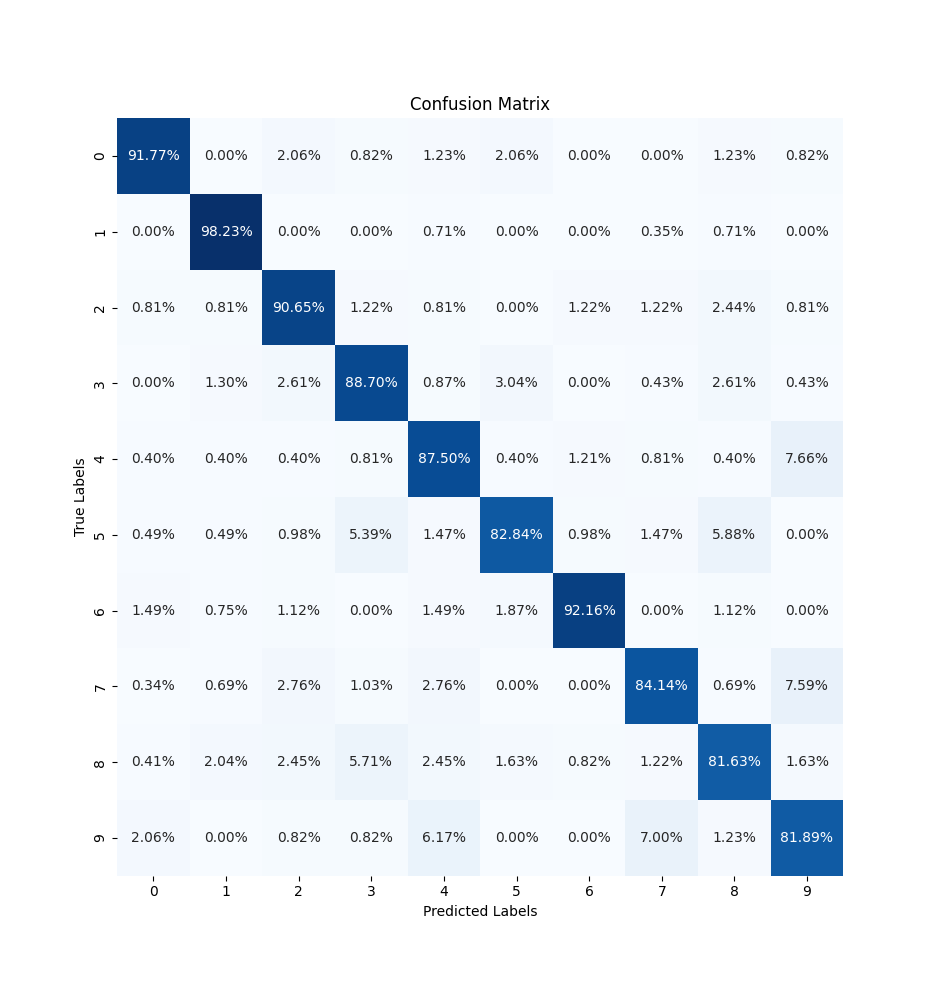
\includegraphics[width=0.9\textwidth, height=0.75\textwidth]{conf_mat_mnist28.png}
	\caption{Development of the prediction accuracy with the progression of epochs}
  \label{fig:MINST_conf}
\end{figure}


\end{document}
